\documentclass[12pt,a4paper]{article}

% The report is designed for Tectonic's XeTeX engine and Overleaf.
\usepackage{fontspec}
\setmainfont{Liberation Serif}
\setmonofont{Liberation Mono}[Scale=MatchLowercase]
\usepackage[english]{babel}
\usepackage[left=2cm,right=1.5cm,top=2cm,bottom=2cm]{geometry}
\usepackage{setspace}
\usepackage{graphicx}
\usepackage{xcolor}
\usepackage{listings}
\usepackage{fancyvrb}
\usepackage{titlesec}
\usepackage{caption}
\usepackage{float}
\usepackage{array}
\usepackage{booktabs}
\usepackage{tikz}
\usetikzlibrary{arrows.meta,positioning,fit}
\usepackage[hidelinks]{hyperref}

\graphicspath{{figures/}}
\onehalfspacing
\setlength{\parindent}{1.25cm}
\setlength{\parskip}{0pt}
\setlength{\emergencystretch}{2em}

% All numbers of the text come from the files in data/ (made by plots/make_figures.py).
% made by plots/make_figures.py - do not edit
\newcommand{\badFloodErrors}{1035}
\newcommand{\badFloodWorstMs}{5.3}
\newcommand{\badRandomErrors}{11}
\newcommand{\checksFailed}{0}
\newcommand{\checksPassed}{80}
\newcommand{\checksScenarios}{15}
\newcommand{\checksTotal}{80}
\newcommand{\consAccepted}{126}
\newcommand{\consClients}{4}
\newcommand{\consDeliveries}{300}
\newcommand{\consOrders}{400}
\newcommand{\consReady}{0}
\newcommand{\consRefused}{274}
\newcommand{\consStock}{194}
\newcommand{\consStockAfter}{320}
\newcommand{\envCores}{2}
\newcommand{\envDate}{2026-11-17}
\newcommand{\envDotnet}{10.0.115}
\newcommand{\envKernel}{6.18.44-fc-v553}
\newcommand{\envLogical}{2}
\newcommand{\envMemory}{7.8}
\newcommand{\envOs}{Ubuntu 24.04.5 LTS}
\newcommand{\envProcessor}{Intel(R) Xeon(R) Processor @ 2.10GHz}
\newcommand{\envPython}{3.13.18}
\newcommand{\envThreadsPerCore}{1}
\newcommand{\fourCloseMs}{6}
\newcommand{\fourFreedSeconds}{2.02}
\newcommand{\fourKillMs}{5}
\newcommand{\fourResetMs}{21}
\newcommand{\idleClientsMax}{1000}
\newcommand{\idleKbPerClient}{33}
\newcommand{\idleMemMax}{63.2}
\newcommand{\idleMemZero}{31.0}
\newcommand{\idleMenuMs}{0.046}
\newcommand{\idleThreadsMax}{1013}
\newcommand{\idleThreadsZero}{14}
\newcommand{\muteSeconds}{5.5}
\newcommand{\muteSent}{635000}
\newcommand{\netRun}{1}
\newcommand{\netSeconds}{24.4}
\newcommand{\oneAnswerMs}{4.4}
\newcommand{\oneReadySeconds}{11.00}
\newcommand{\raceAccepted}{70}
\newcommand{\raceClients}{20}
\newcommand{\raceCroissants}{7}
\newcommand{\raceOrders}{200}
\newcommand{\raceRefused}{130}
\newcommand{\raceRounds}{10}
\newcommand{\restartAfter}{coffee=48 tea=27 croissant=38}
\newcommand{\restartFirst}{coffee=48 tea=22 croissant=39}
\newcommand{\threeAlertMs}{1.1}
\newcommand{\twoEndpoints}{\texttt{127.0.0.1:55540}, \texttt{127.0.0.1:55544}, \texttt{127.0.0.1:55558}, \texttt{127.0.0.1:55568}, \texttt{127.0.0.1:55582}}
\newcommand{\twoMenuMs}{0.9}
\newcommand{\twoOrders}{6}
\newcommand{\twoSeconds}{11.0}
\newcommand{\workCpuMax}{90}
\newcommand{\workOrders}{8}
\newcommand{\workSecondsEight}{2.0}
\newcommand{\workSecondsFour}{4.0}
\newcommand{\workSecondsOne}{16.0}
\newcommand{\workSecondsSixteen}{2.0}
\newcommand{\workSecondsTwo}{8.0}


\definecolor{codebackground}{HTML}{F3F4F6}
\definecolor{codeframe}{HTML}{D1D5DB}
\definecolor{commentgreen}{HTML}{3F6212}
\definecolor{keywordblue}{HTML}{1D4ED8}
\definecolor{alertorange}{HTML}{C2410C}

\titleformat{\section}
  {\normalfont\bfseries\centering\fontsize{13}{16}\selectfont}
  {\thesection}{0.8em}{\MakeUppercase}
\titleformat{name=\section,numberless}
  {\normalfont\bfseries\centering\fontsize{13}{16}\selectfont}
  {}{0pt}{\MakeUppercase}
\titleformat{\subsection}
  {\normalfont\bfseries\fontsize{12}{15}\selectfont}
  {\thesubsection}{0.7em}{}
\titlespacing*{\section}{0pt}{0pt}{12pt}
\titlespacing*{\subsection}{0pt}{10pt}{6pt}

\lstdefinestyle{csharp}{
  language=[Sharp]C,
  basicstyle=\ttfamily\footnotesize,
  keywordstyle=\color{keywordblue}\bfseries,
  commentstyle=\color{commentgreen},
  backgroundcolor=\color{codebackground},
  frame=single,
  rulecolor=\color{codeframe},
  breaklines=true,
  columns=fullflexible,
  keepspaces=true,
  showstringspaces=false,
  numbers=left,
  numberstyle=\tiny\color{gray},
  escapeinside={(*@}{@*)},
  xleftmargin=0.5cm,
  framexleftmargin=0.4cm,
  aboveskip=7pt,
  belowskip=7pt
}

% transcripts of the clients and logs of the server, included from tables/excerpt_*.txt
\lstdefinestyle{log}{
  basicstyle=\ttfamily\fontsize{8.5}{10}\selectfont,
  frame=single,
  rulecolor=\color{codeframe},
  breaklines=true,
  columns=fullflexible,
  keepspaces=true,
  showstringspaces=false,
  upquote=true,
  aboveskip=7pt,
  belowskip=7pt
}

\DefineVerbatimEnvironment{terminaloutput}{Verbatim}{
  fontsize=\footnotesize,
  frame=single,
  framesep=3mm,
  rulecolor=\color{codeframe}
}

\begin{document}

% -----------------------------------------------------------------------------
% Title page
% -----------------------------------------------------------------------------
\begin{titlepage}
  \begin{center}
    \IfFileExists{figures/LOGO_UTM.jpg}{%
      
\includegraphics[width=3.4cm]{figures/LOGO_UTM.jpg}\par
      \vspace{0.25cm}
    }{}

    {\bfseries\fontsize{14}{17}\selectfont
      MINISTRY OF EDUCATION AND RESEARCH\par
      OF THE REPUBLIC OF MOLDOVA\par
      Technical University of Moldova\par
      Faculty of Computers, Informatics and Microelectronics\par
      Department of Software Engineering and Automation\par
    }

    \vspace{0.8cm}
    {\bfseries\fontsize{16}{19}\selectfont
      Moisei Daniel, FAF-241\par
      Strulea Teodor, FAF-242\par}

    \vspace{0.8cm}
    {\bfseries\fontsize{36}{40}\selectfont Report\par}
    \vspace{0.25cm}
    {\itshape\fontsize{20}{24}\selectfont Laboratory Work No. 2\par}
    {\bfseries\itshape\fontsize{20}{24}\selectfont Network Programming (PR)\par}

    \vspace{0.7cm}
    {\fontsize{20}{25}\selectfont Topic: A Coffee Shop Server\par}
    \vspace{0.2cm}
    {\fontsize{15}{19}\selectfont TCP Sockets, Worker Threads, Shared State\par}
  \end{center}

  \vfill
  \begin{flushright}
    {\fontsize{15}{18}\selectfont Checked by:}\par
    \textbf{Fi\c{s}tic Cristofor}, \textit{assistant lecturer}
  \end{flushright}

  \vfill
  \begin{center}
    {\bfseries\fontsize{14}{17}\selectfont Chi\c{s}in\u{a}u -- 2026}
  \end{center}
\end{titlepage}

\pagenumbering{arabic}
\setcounter{page}{2}
\tableofcontents
\newpage

\section*{Introduction}
\addcontentsline{toc}{section}{Introduction}

The purpose of this laboratory work is to build the server of a coffee shop directly on TCP sockets. Clients order coffee, tea and croissants; the server takes the products from a shared stock, prepares the orders with a fixed number of workers and tells every client when its order is ready. A provider brings new products and is alerted when a product runs low. The server has to serve many clients at the same time, protect the data they share, and keep running when a client fails or sends nonsense.

The work was done jointly by Moisei Daniel (FAF-241) and Strulea Teodor (FAF-242). The program is written in C\# (.NET 10) and uses only the class \texttt{Socket}; \texttt{TcpListener}, \texttt{TcpClient} and \texttt{NetworkStream} are not used. It continues the style of Laboratory Work~1: threads are created with \texttt{new Thread}, shared data is protected with \texttt{lock}, and the orders pass from the clients to the workers through a blocking queue. One program starts as the server, a client or the provider, chosen by its first argument.

The report first describes the protocol and the implementation, then goes through the four tasks, answering the questions of each one, and ends with the control questions. Every claim about the behaviour of the server is backed by a scenario that was run against the real server: the transcripts, the server logs and all numbers in the text are produced from those runs by a script, in the same way as the tables of Laboratory Work~1.

\newpage
\section{Short Theory}

\subsection{Listening Socket and Connected Sockets}

A server creates one socket, binds it to a port and calls \texttt{Listen}: this is the \textit{listening socket}. No data of a client ever passes through it; it only receives requests for new connections. Each call of \texttt{Accept} returns a new, \textit{connected} socket for exactly one client. A connection is identified by four values: the address and port of the client and the address and port of the server. All connected sockets of the server share its port; they differ by the address and port of the other side.

\subsection{TCP Is a Stream of Bytes}

TCP delivers the bytes in order and without loss, but it does not keep the borders of the messages. What one side sends with one \texttt{Send} can arrive in two calls of \texttt{Receive}, and two messages that were sent separately can arrive together. The program must mark by itself where a message ends; the two usual ways are a length in front of the message or a delimiter at its end. We use a delimiter: every message is one line of text that ends with \texttt{\textbackslash n}.

\subsection{How a Connection Ends}

There are three ways, and the server sees them differently. When the other side closes the connection in the normal way, its system sends a FIN and \texttt{Receive} returns 0: the end of the stream. When the other side has abandoned the connection (for example, a process was killed while unread data waited in its socket), its system sends an RST and \texttt{Receive} fails with the error \textit{connection reset}. When the other side simply becomes silent, because its cable was pulled or the machine lost power, nothing arrives at all, and a blocked \texttt{Receive} waits for ever unless something makes it stop.

\subsection{Producers, Consumers and Shared State}

The pattern of Task~1c of Laboratory Work~1 appears again: some threads produce work, other threads consume it, and a queue stands between them, so that the producers do not wait for the work to be done. Here the threads of the clients produce orders and the workers consume them. All these threads also read and change the same data (the stock, the orders), so the rule of Laboratory Work~1 applies: a sequence of the form read--check--write on shared data must be exclusive, otherwise two threads can both act on a value that the other one has just changed.

\section{Environment and Test Method}

\subsection{Hardware and Software}

Table~\ref{tab:hardware} describes the machine on which the scenarios of this report were run on \envDate{}; it is written by the test script into \texttt{data/environment.txt}. The clients and the server ran on the same machine and talked through the loopback interface (\texttt{127.0.0.1}).

\begin{table}[H]
  \centering
  \caption{Hardware and software}
  \renewcommand{\arraystretch}{1.25}
  \begin{tabular}{>{\raggedright\arraybackslash}p{0.27\textwidth}>{\raggedright\arraybackslash}p{0.6\textwidth}}
    \toprule
    \textbf{Item} & \textbf{Value} \\
    \midrule
    Processor & \envProcessor \\
    Logical processors & \envLogical{} (\envThreadsPerCore{} per core) \\
    Memory & \envMemory~GiB RAM \\
    Operating system & \envOs, Linux \envKernel \\
    Language and runtime & C\# on .NET SDK \envDotnet, Release build \\
    Test clients & Python \envPython{} (module \texttt{socket}) \\
    \bottomrule
  \end{tabular}
  \label{tab:hardware}
\end{table}

\subsection{Scenarios}

The console client is good for showing the shop by hand, but it cannot send half a message, send random bytes, order from twenty connections at the same instant or stop reading. For this reason the checks are made by a script, \texttt{tests/scenarios.py}. Its clients are plain Python sockets; a thread for each of them records every received line with the time of its arrival. For every scenario the script starts a fresh server process, runs the clients, compares what happened with what must happen, and saves the transcript of the clients and the log of the server.

Two settings of the scenarios differ from a normal start of the server. First, they start it with \texttt{-{}-workers 2}, so that ``more clients than workers'' needs only three clients on any machine; without this option the server creates one worker for each logical processor (\envLogical{} on this machine). Second, most scenarios give the server a known stock (12 coffees, 30 teas, 7 croissants) through its stock file, so that the expected answers are fixed; the random stock of a normal start is checked separately (Section~\ref{sec:bonus}).

Table~\ref{tab:checks} lists the scenarios. In the run used for this report \checksPassed{} of \checksTotal{} checks passed. In the transcripts below, \texttt{A >} is a message sent by client A, \texttt{A <} a message that A received, and the number in front is the time in seconds from the start of the scenario.

\begin{table}[H]
  \centering
  \caption{The scenarios of \texttt{tests/scenarios.py} and their checks}
  \small
  \begin{tabular}{lllr}
\toprule
Scenario & For & What it tries & Checks passed \\
\midrule
\texttt{task1} & Task 1 & menu, order, refusal, errors, READY after 11 s & 11 of 11 \\
\texttt{framing} & Task 1 & messages in pieces, several in one send & 4 of 4 \\
\texttt{task2} & Task 2 & five clients, two workers, queue order & 6 of 6 \\
\texttt{race} & Task 2 & 20 simultaneous orders for 7 croissants, 10 rounds & 2 of 2 \\
\texttt{task3} & Task 3 & provider, delivery, alerts & 13 of 13 \\
\texttt{conservation} & Task 3 & deliveries and orders at the same moment & 2 of 2 \\
\texttt{task4} & Task 4 & closed, reset and killed clients & 11 of 11 \\
\texttt{network} & Task 4 & a client whose network is gone & 3 of 3 \\
\texttt{invalid} & Task 4 & wrong commands, long message, random bytes & 17 of 17 \\
\texttt{never\_reads} & Task 4 & a client that never reads & 2 of 2 \\
\texttt{client\_cs} & Task 4 & the console client in C\# & 2 of 2 \\
\texttt{client\_py} & Bonus & the console client in Python & 2 of 2 \\
\texttt{restart} & Bonus & random stock; stock kept after a restart & 3 of 3 \\
\texttt{idle\_clients} & Questions & 1000 idle clients & 1 of 1 \\
\texttt{workers} & Questions & 1 to 16 workers & 1 of 1 \\
\bottomrule
\end{tabular}

  \label{tab:checks}
\end{table}

\newpage
\section{Implementation}

\subsection{Program Structure}

\texttt{Program.cs} chooses the role from the first argument: \texttt{server}, \texttt{client} or \texttt{provider}; the port, and for the client and the provider the address of the server, are options (\texttt{-{}-port}, \texttt{-{}-host}). The server consists of three classes with separate duties. \texttt{Server} owns the listening socket and creates the threads. \texttt{Connection} is one accepted socket with its thread: it receives, understands the messages and sends the answers. \texttt{Shop} holds everything that the threads share and the lock that protects it; it never touches a socket. The helper classes are \texttt{MessageReader} (cuts bytes into messages; used by the server and by the client), \texttt{Menu} and \texttt{Order}, \texttt{Log} and \texttt{Args}. \texttt{Client} is the console program of the client and of the provider.

\subsection{The Protocol}

A message is one line of UTF-8 text that ends with \texttt{\textbackslash n}, at most 1024 bytes long. The first word is the command, in upper or lower case; the other words are its parameters. Table~\ref{tab:protocol} lists all messages. Text was chosen instead of a binary format because it can be typed by hand (also with \texttt{nc}) and read in a log.

\begin{table}[H]
  \centering
  \caption{The messages of the protocol}
  \renewcommand{\arraystretch}{1.2}
  \small
  \begin{tabular}{>{\raggedright\arraybackslash}p{0.33\textwidth}>{\raggedright\arraybackslash}p{0.6\textwidth}}
    \toprule
    \textbf{The client or provider sends} & \textbf{The server answers} \\
    \midrule
    \texttt{MENU} & \texttt{MENU coffee=12 tea=30 croissant=7} \\
    \texttt{ORDER croissant 2 tea 1} & \texttt{ACCEPTED order=7 seconds=7}, or \texttt{REFUSED not enough in stock:} followed by the stock \\
    \texttt{PROVIDER} & \texttt{PROVIDER ok} \\
    \texttt{DELIVER coffee 20 croissant 10} & \texttt{DELIVERED} followed by the new stock (only for the provider) \\
    anything wrong & \texttt{ERROR} followed by what is wrong \\
    \midrule
    \multicolumn{2}{l}{\textbf{The server sends by itself}} \\
    \midrule
    to the client of an order & \texttt{READY order=7}, when a worker has prepared it \\
    to the provider & \texttt{ALERT croissant=3}, when an order leaves a product below 5 \\
    \bottomrule
  \end{tabular}
  \label{tab:protocol}
\end{table}

\subsection{Threads and Sockets of the Server}

Figure~\ref{fig:architecture} shows the server with two clients and the provider. The main thread only accepts. Every connection has its own thread, which spends almost all its time waiting in \texttt{Receive}; this is the simplest way to serve many clients at once, and its cost is measured in Section~\ref{sec:control}. The workers are created once, at the start: \texttt{Environment.ProcessorCount} of them, as the assignment asks.

\begin{figure}[H]
\centering
\caption{Threads (blue frames), shared data (grey) and sockets of the server}
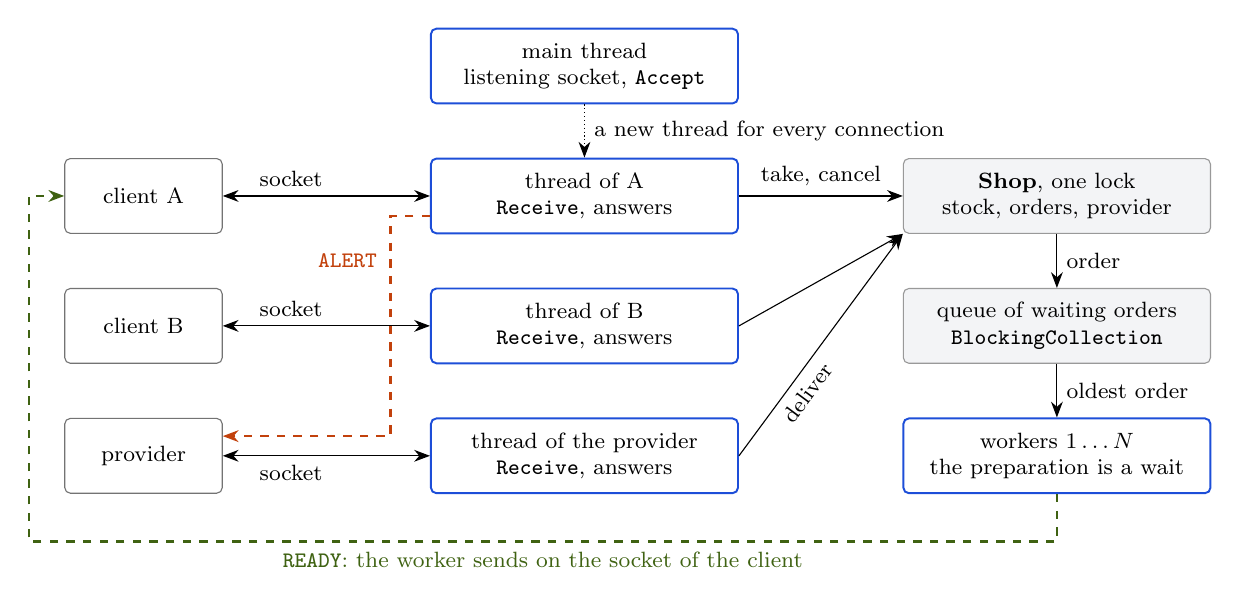
\begin{tikzpicture}[font=\footnotesize, >={Stealth[length=2mm]},
  box/.style={draw=codeframe, rounded corners=2pt, align=center, inner sep=4pt, minimum height=0.95cm},
  thr/.style={box, fill=white, draw=keywordblue, line width=0.7pt, minimum width=3.9cm},
  ext/.style={box, fill=white, draw=black!55, minimum width=2.0cm},
  data/.style={box, fill=codebackground, draw=black!40, minimum width=3.9cm}]
  \node[ext] (a) at (0,3.3) {client A};
  \node[ext] (b) at (0,1.65) {client B};
  \node[ext] (p) at (0,0) {provider};

  \node[thr] (main) at (5.6,4.95) {main thread\\listening socket, \texttt{Accept}};
  \node[thr] (ta) at (5.6,3.3) {thread of A\\\texttt{Receive}, answers};
  \node[thr] (tb) at (5.6,1.65) {thread of B\\\texttt{Receive}, answers};
  \node[thr] (tp) at (5.6,0) {thread of the provider\\\texttt{Receive}, answers};

  \node[data] (shop) at (11.6,3.3) {\textbf{Shop}, one lock\\stock, orders, provider};
  \node[data] (queue) at (11.6,1.65) {queue of waiting orders\\\texttt{BlockingCollection}};
  \node[thr] (w) at (11.6,0) {workers $1 \dots N$\\the preparation is a wait};

  \draw[<->] (a) -- node[above, pos=0.33]{socket} (ta);
  \draw[<->] (b) -- node[above, pos=0.33]{socket} (tb);
  \draw[<->] (p) -- node[below, pos=0.33]{socket} (tp);
  \draw[->, densely dotted] (main) -- node[right]{a new thread for every connection} (ta);

  \draw[->] (ta) -- node[above]{take, cancel} (shop);
  \draw[->] (tb.east) -- (shop.south west);
  \draw[->] (tp.east) -- node[below, sloped, pos=0.33]{deliver} (shop.south west);
  \draw[->] (shop) -- node[right]{order} (queue);
  \draw[->] (queue) -- node[right]{oldest order} (w);

  \draw[->, dashed, commentgreen, line width=0.8pt] (w.south) -- ++(0,-0.6) -| node[pos=0.25, below]{\texttt{READY}: the worker sends on the socket of the client} ([xshift=-0.45cm]a.west) -- (a.west);
  \draw[->, dashed, alertorange, line width=0.8pt] ([yshift=-0.25cm]ta.west) -- ++(-0.5,0) |- ([yshift=0.25cm]p.east);
  \node[alertorange, anchor=east] at ([xshift=-0.55cm, yshift=-0.82cm]ta.west) {\texttt{ALERT}};
\end{tikzpicture}
\label{fig:architecture}
\end{figure}

\begin{lstlisting}[style=csharp,caption={The listening socket and the accept loop (Server.cs)}]
Socket listener = new Socket(AddressFamily.InterNetwork, SocketType.Stream,
                             ProtocolType.Tcp);
listener.SetSocketOption(SocketOptionLevel.Socket, SocketOptionName.ReuseAddress, true);
// Any: all addresses of this machine, so the server is also reachable from other computers
listener.Bind(new IPEndPoint(IPAddress.Any, port));
listener.Listen(100);
...
while (true)
{
    Socket client;
    try
    {
        client = listener.Accept();   // waits here; returns a new socket for every client
    }
    catch (SocketException e) { ... continue; }
    ...
    Connection connection = new Connection(client, shop);
    Thread thread = new Thread(connection.Run);
    thread.IsBackground = true;
    thread.Start();
}
\end{lstlisting}

\subsection{Cutting the Bytes into Messages}

Every connection has its own \texttt{MessageReader}. After each \texttt{Receive} the received bytes are given to it. It copies them into a buffer of 1024 bytes for the current line; at every \texttt{\textbackslash n} it reports one complete message and starts a new line. Bytes of an unfinished message simply stay in the buffer until the next \texttt{Receive} brings the rest. If more than 1024 bytes arrive without a line end, the reader reports ``too long'' once, at that moment, and throws away everything up to the next \texttt{\textbackslash n}; the memory used for a connection is therefore fixed, whatever the client sends.

\begin{lstlisting}[style=csharp,caption={MessageReader.Add}]
public void Add(byte[] buffer, int count, Action<string> onMessage, Action onTooLong)
{
    for (int i = 0; i < count; i++)
    {
        byte b = buffer[i];

        if (b == '\n')
        {
            if (!skipping)
                onMessage(Encoding.UTF8.GetString(line, 0, length).TrimEnd('\r'));
            length = 0;
            skipping = false;
        }
        else if (skipping)
        {
            // still inside the message that was too long
        }
        else if (length == MaxLength)
        {
            skipping = true;
            onTooLong();
        }
        else
        {
            line[length] = b;
            length++;
        }
    }
}
\end{lstlisting}

\subsection{The Shared State and Its Lock}

All shared data of the shop is in the class \texttt{Shop}, and every method of it takes the same lock, \texttt{gate}. An order is handled in one critical section: the stock is checked for all products of the order, and only if all are available they are taken, the order gets its number and is registered for its client. Two rules keep the critical sections short. Nothing is sent to a socket inside the lock, so a slow client cannot stop the shop; the method returns copies of the data (\texttt{stockNow}) that the caller uses after the lock is released.

\begin{lstlisting}[style=csharp,caption={Checking and taking in one step (Shop.cs)}]
public Order? TakeOrder(Connection client, int[] items, out int[] stockNow)
{
    lock (gate)
    {
        bool enough = true;
        for (int i = 0; i < Menu.Count; i++)
        {
            if (items[i] > stock[i])
                enough = false;
        }

        if (!enough)
        {
            stockNow = (int[])stock.Clone();
            return null;
        }

        for (int i = 0; i < Menu.Count; i++)
            stock[i] -= items[i];
        SaveStock();

        Order order = new Order(nextNumber, client, items);
        nextNumber++;
        client.Orders.Add(order);

        stockNow = (int[])stock.Clone();
        return order;
    }
}
\end{lstlisting}

The thread of the client then answers and passes the order to the workers. The answer is sent before the order enters the queue, so \texttt{READY} can never arrive before \texttt{ACCEPTED}.

\begin{lstlisting}[style=csharp,caption={An accepted order (Connection.HandleOrder)}]
Order? order = shop.TakeOrder(this, items, out int[] stockNow);
if (order == null)
{
    Log.Write(Name, $"order refused: ...");
    Send("REFUSED not enough in stock: " + Menu.Format(stockNow));
    return;
}

Log.Write(Name, $"order {order.Number} accepted: ...");
Send($"ACCEPTED order={order.Number} seconds={order.Seconds}");
shop.Enqueue(order);

shop.AlertProvider(items);
\end{lstlisting}

\subsection{The Workers}

A worker repeats four steps: take the oldest order from the queue (it waits there while the queue is empty), mark it as being prepared, wait for the preparation time, mark it as ready and tell the client. The wait is not \texttt{Thread.Sleep} but a wait on an event of the connection, \texttt{Gone}, with the preparation time as its limit: it ends earlier when the client disappears (Section~\ref{sec:task4}). The state of an order is changed only inside the lock of the shop, by \texttt{StartPreparing} and \texttt{Finish}; both return \texttt{false} when the order was cancelled meanwhile.

\begin{lstlisting}[style=csharp,caption={A worker (Server.Work)}]
while (true)
{
    Order order = shop.TakeNext();   // waits here while the queue is empty
    try
    {
        if (!shop.StartPreparing(order))
            continue;   // cancelled while it waited in the queue

        Log.Write(order.Client.Name, $"order {order.Number}: worker {number} prepares it ...");

        // The preparation is simulated by waiting.
        // The wait ends earlier when the client disappears.
        order.Client.Gone.Wait(TimeSpan.FromSeconds(order.Seconds));

        if (shop.Finish(order))
        {
            Log.Write(order.Client.Name, $"order {order.Number} ready (worker {number})");
            order.Client.Send($"READY order={order.Number}");
        }
        else
        {
            Log.Write(order.Client.Name, $"order {order.Number}: worker {number} stopped ...");
        }
    }
    catch (Exception e) { ... }   // a mistake in our code must not end the worker
}
\end{lstlisting}

\subsection{Sending from Several Threads}

Three kinds of threads can send on the same socket: the thread of the connection (answers), a worker (\texttt{READY}) and, for the provider, the thread of any client (\texttt{ALERT}). \texttt{Connection.Send} is the only place that sends, and it holds a lock of that connection while the bytes of one message go out. A failed send does not clean up anything: it closes the socket, and the thread of the connection, which then leaves \texttt{Receive} with an error, does the cleanup. In this way the cleanup has one owner and cannot run twice.

\begin{lstlisting}[style=csharp,caption={Connection.Send}]
public void Send(string message)
{
    if (closed)
        return;

    byte[] bytes = Encoding.UTF8.GetBytes(message + "\n");
    try
    {
        lock (sendGate)
        {
            // Send can take only a part of the bytes: it is repeated until all are sent
            int sent = 0;
            while (sent < bytes.Length)
                sent += socket.Send(bytes, sent, bytes.Length - sent, SocketFlags.None);
        }
    }
    catch (Exception e) when (e is SocketException or ObjectDisposedException)
    {
        // The client is gone, or it has not read for 5 seconds (SendTimeout).
        // The socket is closed here; the thread of the connection then leaves Receive
        // and cancels the orders.
        if (!closed)
            Log.Write(Name, $"error: send failed (...), the server closes the connection");
        Close();
    }
}
\end{lstlisting}

\subsection{The Provider and the Alerts}

A connection becomes the provider by sending \texttt{PROVIDER}; the shop remembers this connection (inside the lock) and refuses a second provider while the first is connected. \texttt{AlertProvider} is called with a list of products and sends an alert for each of them that is below 5 at that moment. It is called from two places: by the thread of a client right after its order took products, and by the thread of the provider when it has just connected, for all products. The second call is what delivers the alerts that nobody received while no provider was connected: instead of storing old alerts, the server looks at the stock as it is now, so an alert that is no longer true (a client left and its products came back) is not sent.

\begin{lstlisting}[style=csharp,caption={Shop.AlertProvider}]
public void AlertProvider(int[] products)
{
    lock (alertGate)   // one alert at a time: two alerts cannot overtake each other
    {
        Connection? to;
        int[] now;
        lock (gate)
        {
            to = provider;
            now = (int[])stock.Clone();
        }

        if (to == null)
            return;

        for (int i = 0; i < Menu.Count; i++)
        {
            if (products[i] > 0 && now[i] < LowStock)
            {
                Log.Write(to.Name, $"alert sent to the provider: {Menu.Names[i]}={now[i]}");
                to.Send($"ALERT {Menu.Names[i]}={now[i]}");
            }
        }
    }
}
\end{lstlisting}

\subsection{When a Client Disappears}
\label{sec:leave}

The thread of a connection leaves its receive loop in three cases: \texttt{Receive} returned 0, \texttt{Receive} failed, or the socket was closed by another thread after a failed send. In all of them the same lines run. \texttt{Shop.Leave} cancels, inside the lock, every unfinished order of the client, whether it waits in the queue or is at a worker, and puts its products back; then the event \texttt{Gone} is set, which wakes a worker that is preparing one of these orders.

\begin{lstlisting}[style=csharp,caption={The end of Connection.Run and Shop.Leave}]
// First the orders are cancelled inside the lock of the shop, then the worker is woken:
// when it looks at its order, the order is already cancelled.
List<string> cancelled = shop.Leave(this);
foreach (string line in cancelled)
    Log.Write(Name, line);

Gone.Set();
Close();
...
public List<string> Leave(Connection client)
{
    List<string> cancelled = new List<string>();
    lock (gate)
    {
        foreach (Order order in client.Orders)
        {
            string where = order.State == OrderState.Preparing
                ? "was being prepared" : "waited in the queue";
            order.State = OrderState.Cancelled;

            for (int i = 0; i < Menu.Count; i++)
                stock[i] += order.Items[i];

            cancelled.Add($"order {order.Number} cancelled ({where}): ...");
        }
        ...
        if (provider == client)
            provider = null;
    }
    return cancelled;
}
\end{lstlisting}

A client whose network is gone sends nothing, so \texttt{Receive} alone would never end. Every accepted socket therefore gets TCP keep-alive with short times, and a limit for sending:

\begin{lstlisting}[style=csharp,caption={Options of an accepted socket (Server.Prepare)}]
client.SendTimeout = 5000;
client.SetSocketOption(SocketOptionLevel.Socket, SocketOptionName.KeepAlive, true);
client.SetSocketOption(SocketOptionLevel.Tcp, SocketOptionName.TcpKeepAliveTime, 10);
client.SetSocketOption(SocketOptionLevel.Tcp, SocketOptionName.TcpKeepAliveInterval, 5);
client.SetSocketOption(SocketOptionLevel.Tcp, SocketOptionName.TcpKeepAliveRetryCount, 3);
\end{lstlisting}

\subsection{The Client and the Provider}

The console program has two threads. The main thread receives and prints every message with the time of its arrival. A second thread reads the keyboard and sends each typed line as a message; only \texttt{help} and \texttt{quit} are handled locally, everything else, also a wrong command, goes to the server. The keyboard thread is a background thread, so the program ends as soon as the main thread ends. The provider is the same program; it sends \texttt{PROVIDER} right after it has connected.

\begin{lstlisting}[style=csharp,caption={The two threads of Client.cs}]
// a background thread does not keep the program alive: when the main thread ends,
// the program ends, also while this thread still waits in Console.ReadLine
Thread keyboard = new Thread(() => ReadKeyboard(isProvider));
keyboard.IsBackground = true;
keyboard.Start();

try
{
    byte[] buffer = new byte[4096];
    MessageReader reader = new MessageReader();
    while (true)
    {
        int count = socket.Receive(buffer);   // waits here for the server
        if (count == 0)
        {
            Console.WriteLine(quitting ? "Bye." : "The server closed the connection.");
            break;
        }
        reader.Add(buffer, count, Show, () => Show("(a message that was too long)"));
    }
}
catch (SocketException e)
{
    Console.WriteLine($"The connection to the server was lost ({e.SocketErrorCode}).");
}
socket.Close();
\end{lstlisting}

\subsection{Tools Used and Why}

As in Laboratory Work~1, for every need we used the simplest tool that does it; the alternatives that were not used are named, with the reason.

\textbf{Sockets.} \texttt{Socket} with \texttt{Bind}, \texttt{Listen}, \texttt{Accept}, \texttt{Connect}, \texttt{Send}, \texttt{Receive}, \texttt{Shutdown} and \texttt{Close}, in blocking mode. The option \texttt{ReuseAddress} lets the server start again on the same port right after it was stopped. The client resolves a host name with \texttt{Dns.GetHostAddresses}, which is not a wrapper of the socket.

\textbf{One thread for each connection.} A blocking \texttt{Receive} needs somebody who waits in it, and with a thread for each connection the code of one client is a plain loop. \texttt{Socket.Select} or the asynchronous methods (\texttt{ReceiveAsync} with \texttt{await}) would serve many connections with few threads, but the code becomes harder to follow, and for the number of clients of a coffee shop the threads cost little (Section~\ref{sec:control}). The thread pool was not used for the connections for the reason found in Laboratory Work~1: these threads block almost all the time, and a blocked pool thread serves nobody.

\textbf{\texttt{lock}.} One lock for the whole shop. The stock, the state of the orders and the provider change together (an order changes the stock and the list of orders; a client that leaves changes the states and the stock), so one lock keeps them consistent and cannot deadlock with itself. Separate locks for every product would allow two orders for different products to run at the same time, but an order for several products would have to take several locks in a fixed order, and the critical sections are short. The longest part of one is the writing of the small stock file, which is done inside the lock on purpose, so that the file always holds the same stock as the memory. \texttt{Interlocked} is enough for one number, not for ``check three numbers and then change them''.

\textbf{\texttt{BlockingCollection<Order>}.} The queue between the clients and the workers, as in Task~1c of Laboratory Work~1: \texttt{Take} waits while it is empty, and it keeps the order of arrival. It has no size limit here, because an order enters it only after its products were taken from the stock, so the stock limits the number of waiting orders. An order cannot be removed from the middle of this queue; a cancelled order stays there, already cancelled, and the worker that takes it skips it.

\textbf{\texttt{ManualResetEventSlim}.} The event \texttt{Gone} of a connection. A worker needs ``wait $n$ seconds, or less if the client disappears''; \texttt{Thread.Sleep} cannot be interrupted in a clean way, and a loop that sleeps a little and looks at a flag wakes up late and wastes work. \texttt{Wait} with a time limit does exactly this, and one event serves all orders of the client.

\textbf{\texttt{volatile bool}.} Two flags that one thread sets and another reads, without any other data depending on them: \texttt{closed} of a connection and \texttt{quitting} of the client. A lock would also work; \texttt{volatile} is enough for a single flag that is only set once.

\textbf{TCP keep-alive and \texttt{SendTimeout}.} Both are options of the socket, so no thread of ours has to watch the clients. An own \texttt{PING} message would do the same, but it needs a timer and one more message in the protocol.

\newpage
\section{Task 1: One Client}

The scenario \texttt{task1} uses one client. Listing~\ref{lst:task1} is its transcript and Listing~\ref{lst:task1log} the log that the server wrote at the same time: a line for the connection, for every accepted and refused order, for every error and for the ready order, each with the endpoint of the client.

\lstinputlisting[style=log,caption={Task 1: what the client sent and received},label={lst:task1}]{tables/excerpt_task1_clients.txt}

\lstinputlisting[style=log,caption={Task 1: the log of the server},label={lst:task1log}]{tables/excerpt_task1_server.txt}

The order for 2 croissants, 1 tea and 1 coffee was answered \oneAnswerMs~ms after it was sent, with its number and $2\cdot2+3+4=11$ seconds. The menu asked right after it already shows the smaller stock. \texttt{READY} arrived by itself \oneReadySeconds~s after \texttt{ACCEPTED}. The order for 6 croissants, when 5 were left, was refused with the stock, and nothing was taken. An unknown product and the quantities \texttt{0}, \texttt{-1}, \texttt{two} and \texttt{1.5} each got an error message.

\textbf{1. How does your code cut the received bytes into messages? What does it do when a message arrives in two pieces, or two messages arrive in one receive?} A message ends with \texttt{\textbackslash n}. The \texttt{MessageReader} of the connection goes through the received bytes one by one and collects them in a line buffer; at each \texttt{\textbackslash n} the collected line is one message. A message in two pieces: the first \texttt{Receive} brings bytes without a line end, they stay in the buffer and nothing is answered; the second \texttt{Receive} brings the rest, and the message is handled then. Two messages in one receive: the loop meets two line ends and handles two messages, one after the other. Listing~\ref{lst:framing} shows the three cases against the server: \texttt{ME} and, half a second later, \texttt{NU\textbackslash n} got one answer, after the second piece; three messages in one send got three answers in the right order (the menu after the order already has one tea less); a message sent byte by byte got one answer.

\lstinputlisting[style=log,caption={Messages in pieces and several messages in one send},label={lst:framing}]{tables/excerpt_framing.txt}

\textbf{2. Why does the server answer at once, and tell the client later that the order is ready? What would the client see otherwise?} The preparation lasts seconds, the decision does not. Whether the order is accepted is known as soon as the stock was checked, so the client is told then, with the time it will have to wait. If the server answered only when the order is ready, the client would see nothing for 11 seconds, and it could not tell an accepted order from a refused one that is slow, from a lost message or from a dead server. The thread of the connection would also be busy waiting instead of receiving: the client could not ask for the menu or order again meanwhile, and the server would notice a client that left only after the wait. With the answer at once and \texttt{READY} later, the thread of the connection is free again after a few milliseconds, and the waiting is done by a worker.

\newpage
\section{Task 2: Many Clients}

\subsection{More Clients Than Workers}

In the scenario \texttt{task2} five clients order within half a second while the server has two workers; a little later client D orders a second time. Figure~\ref{fig:task2} is drawn from the log of the server and Listing~\ref{lst:task2} is the transcript of the clients.

\begin{figure}[H]
\centering
\caption{Task 2: when every order waited and when it was prepared (from the log of the server)}
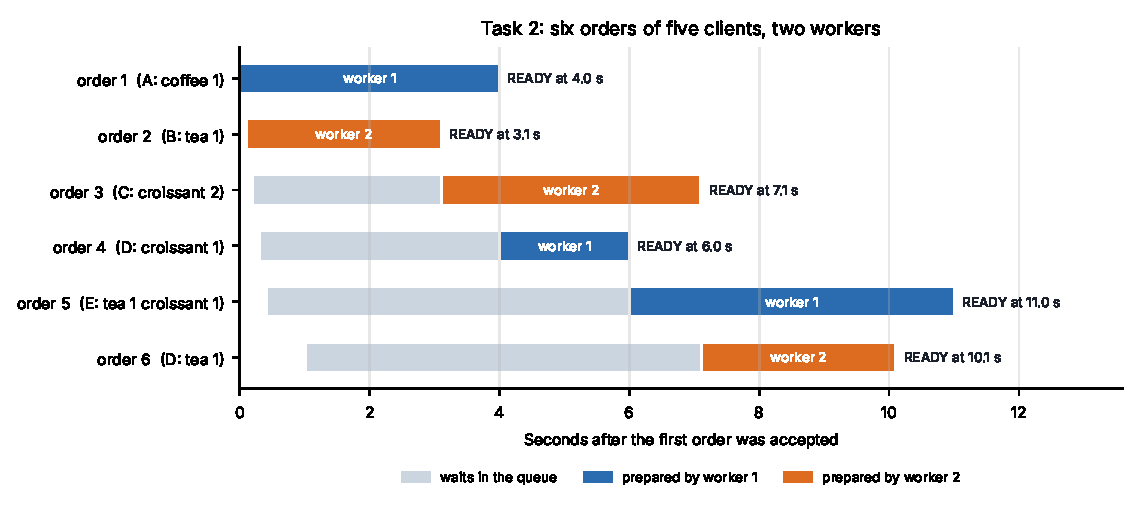
\includegraphics[width=\textwidth]{task2.pdf}
\label{fig:task2}
\end{figure}

\lstinputlisting[style=log,caption={Task 2: five clients and two workers},label={lst:task2}]{tables/excerpt_task2_clients.txt}

All \twoOrders{} orders were accepted at once, although only two could be prepared. Never more than two orders were in preparation at the same time, and the waiting orders were started in the order of their numbers, each one at the moment a worker became free. While both workers were busy, client C asked for the menu and was answered in \twoMenuMs~ms, and client D, which was still waiting for order~4, placed order~6. The last order was ready \twoSeconds~s after the first one was started.

\subsection{The Last Croissant}

The scenario \texttt{race} repeats the dangerous moment many times. The stock has \raceCroissants{} croissants. \raceClients{} threads, each with its own connection, wait at a barrier and then all send \texttt{ORDER croissant 1} together. After the answers the clients leave without waiting, so their croissants come back, and the next round starts; there are \raceRounds{} rounds.

\lstinputlisting[style=log,caption={Twenty simultaneous orders for seven croissants, ten rounds},label={lst:race}]{tables/excerpt_race.txt}

In every round exactly \raceCroissants{} orders were accepted and the others refused: of \raceOrders{} orders, \raceAccepted{} were accepted and \raceRefused{} refused. The stock was 0 after each round, never negative, the accepted orders of a round had different numbers, and after the clients left the stock was \raceCroissants{} again every time. Such a test cannot prove that a race is impossible; it shows that the race did not happen in \raceOrders{} attempts, and the reason why it cannot happen is the lock around the check and the taking.

\subsection{Questions}

\textbf{1. Which data is shared between threads in your server, and how is each of them protected?} Table~\ref{tab:shared} lists everything that more than one thread touches. The receive buffer, the \texttt{MessageReader} and the flag \texttt{isProvider} of a connection are used only by the thread of that connection and need no protection.

\begin{table}[H]
  \centering
  \caption{Shared data of the server}
  \renewcommand{\arraystretch}{1.2}
  \small
  \begin{tabular}{>{\raggedright\arraybackslash}p{0.25\textwidth}>{\raggedright\arraybackslash}p{0.36\textwidth}>{\raggedright\arraybackslash}p{0.30\textwidth}}
    \toprule
    \textbf{Data} & \textbf{Threads that use it} & \textbf{Protection} \\
    \midrule
    The stock & threads of the clients (menu, order, leaving), thread of the provider (delivery) & \texttt{lock (gate)} in \texttt{Shop} \\
    The number of the next order & threads of the clients & the same lock \\
    The state of every order & thread of its client (cancel), a worker (start, finish) & the same lock \\
    The list of unfinished orders of every client & thread of the client (add, cancel), a worker (remove when ready) & the same lock \\
    Who the provider is & thread of the provider (set, clear), threads of the clients (alert) & the same lock \\
    The file with the stock & every thread that changes the stock & written inside the same lock \\
    The queue of orders & threads of the clients (add), workers (take) & \texttt{BlockingCollection} is safe for many threads \\
    Every connected socket, for sending & thread of the connection, workers, threads of other clients (alert) & \texttt{lock (sendGate)} of the connection \\
    The order of the alerts & threads of the clients, thread of the provider & \texttt{lock (alertGate)} \\
    The event \texttt{Gone} and the flag \texttt{closed} of a connection & thread of the connection, workers & the event is safe for many threads; the flag is \texttt{volatile} \\
    The log & all threads & \texttt{Console.WriteLine} writes a whole line at once \\
    \bottomrule
  \end{tabular}
  \label{tab:shared}
\end{table}

\textbf{2. Two clients order the last croissant at the same moment. Show, step by step, what could go wrong without your protection.} The stock has 1 croissant; the threads of clients A and B both handle \texttt{ORDER croissant 1}. (1)~Thread A reads the stock: 1, enough. (2)~Thread B reads the stock: 1, enough. (3)~A writes $1-1=0$. (4)~B writes: 0 if it uses the value it read before, $-1$ if it reads again. (5)~Both send \texttt{ACCEPTED}. Two croissants were sold and one existed; the stock is wrong for every later order. With the lock, steps 1 and 3 of A are one unit: B can read only before A started or after A finished, and in the second case it reads 0 and is refused.

\textbf{3. A worker tells a client that its order is ready while the thread of that client is reading from the same connection. What must you take care of?} Reading and writing at the same time is not a problem: one thread in \texttt{Receive} and another in \texttt{Send} on the same socket use the two independent directions of the connection. The care is needed elsewhere. First, there can be two \emph{senders}: the worker sends \texttt{READY} at the moment when the thread of the client sends an answer to a menu request; without \texttt{sendGate} the bytes of the two messages could be mixed. Second, the socket can die under the worker: the client disappears at that very moment and \texttt{Send} throws; the worker catches this, so it lives on and takes the next order, and it does not clean up, because that belongs to the thread of the connection. Third, the client may not be reading at all: \texttt{Send} would then block the worker for ever once the buffers are full, so sending has a limit of 5 seconds, after which the connection is closed (Section~\ref{sec:invalid}). Fourth, the order of the messages: \texttt{ACCEPTED} is sent before the order is put in the queue, so no worker can send \texttt{READY} first.

\textbf{4. Why one worker per CPU core? The workers spend their time waiting: what would happen with twice as many?} One thread for each core is the right number for work that computes: in Laboratory Work~1 the speed-up stopped growing at the number of cores, because a core can run only one computation at a time. Our workers do not compute; a worker that prepares an order is blocked in a wait and uses no processor. With twice as many workers twice as many orders would be in preparation at the same time and the queue would empty twice as fast, at the cost of one more sleeping thread for each worker. We measured it (Table~\ref{tab:workers} and the left chart of Figure~\ref{fig:measurements}): \workOrders{} orders of 2 seconds that arrive together were all ready after \workSecondsOne~s with 1 worker, \workSecondsTwo~s with 2, \workSecondsFour~s with 4 and \workSecondsEight~s with 8, on a machine with \envLogical{} logical processors; the server used at most \workCpuMax~ms of processor time in any of these runs. With 16 workers the time stays \workSecondsSixteen~s, because there are only \workOrders{} orders. So in this server the number of workers is a rule of the shop: it stands for the people behind the counter, the scarce resource that the queue exists for. It would be a technical limit only if the preparation were a real computation.

\begin{table}[H]
  \centering
  \caption{\workOrders{} orders of one croissant (2 s each) arrive together}
  \begin{tabular}{rrrr}
\toprule
Workers & Orders & All ready after (s) & Processor time of the server (ms) \\
\midrule
1 & 8 & 16.02 & 90 \\
2 & 8 & 8.01 & 90 \\
4 & 8 & 4.01 & 50 \\
8 & 8 & 2.01 & 70 \\
16 & 8 & 2.01 & 60 \\
\bottomrule
\end{tabular}

  \label{tab:workers}
\end{table}

\begin{figure}[H]
\centering
\caption{Measurements: the number of workers (left) and the cost of waiting clients (middle and right)}
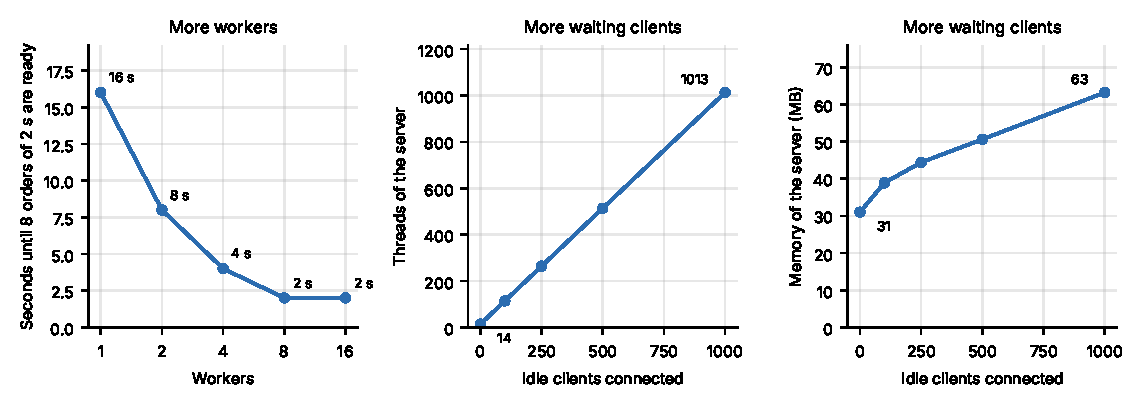
\includegraphics[width=\textwidth]{measurements.pdf}
\label{fig:measurements}
\end{figure}

\newpage
\section{Task 3: The Provider}

In the scenario \texttt{task3} the stock starts with 6 coffees. Listing~\ref{lst:task3} shows the whole exchange; A is a client, P the provider, P2 a second program that claims to be the provider, and P3 a provider that connects after P has left.

\lstinputlisting[style=log,caption={Task 3: deliveries and alerts},label={lst:task3}]{tables/excerpt_task3.txt}

The client that tried to deliver got an error. Its order for 2 coffees left 4 in the stock while no provider was connected; when P connected and said \texttt{PROVIDER}, it received \texttt{ALERT coffee=4} without asking. The next order of the client produced \texttt{ALERT coffee=3} at the provider \threeAlertMs~ms after the client had sent the order. An order for tea, of which 29 were left, produced no alert. The delivery of 20 coffees and 10 croissants was in the stock at once, as the menu of the client shows. A second provider was refused. After P had left, the shop went on accepting orders, and the new provider P3 received the alert for the croissants that nobody had received.

\textbf{1. How does your server know which connection is the provider?} The connection says so: its first message is \texttt{PROVIDER} (the provider program sends it by itself right after connecting). Until then every connection is a client. The server keeps a reference to the provider's connection in the shop, inside the lock, and the connection keeps a flag for itself; \texttt{DELIVER} is accepted only with this flag, and \texttt{ORDER} is refused with it. There is at most one provider: a second \texttt{PROVIDER} gets an error while the first is connected, and the place becomes free when the provider's connection ends. The server believes whoever says \texttt{PROVIDER}; the assignment does not ask for a password, and we did not add one.

\textbf{2. A delivery and an order change the stock at the same moment. Show that no change is lost.} Both changes are made inside \texttt{lock (gate)}: \texttt{Deliver} adds and \texttt{TakeOrder} checks and subtracts, so one of them runs completely before the other starts and no thread can write a value computed from a stock that another thread has changed meanwhile. The scenario \texttt{conservation} tests it: the provider sent \consDeliveries{} deliveries of 1 coffee while \consClients{} clients sent \consOrders{} orders of 1 coffee in total, all at the same time, with 20 coffees at the start. \consAccepted{} orders were accepted and \consRefused{} refused (the orders were faster than the deliveries, so the stock was often empty), and the stock at the end was exactly $20 + \consDeliveries - \consAccepted = \consStock$ (Listing~\ref{lst:conservation}). When the clients then left, their unfinished orders were cancelled and the stock was \consStockAfter.

\lstinputlisting[style=log,caption={Deliveries and orders at the same moment},label={lst:conservation}]{tables/excerpt_conservation.txt}

\textbf{3. Which thread sends the alert to the provider, and when?} The thread of the client whose order made the product fall. After it has taken the products, answered its client and put the order in the queue, it calls \texttt{AlertProvider}, which looks at the stock again and sends \texttt{ALERT} on the socket of the provider, protected by the send lock of that connection. So the alert leaves in the same moment as the order, without any request of the provider and without a timer. The second case is the provider that connects: then its own thread sends the alerts for all products that are below 5 now, right after \texttt{PROVIDER ok}. Because a client thread writes to the socket of somebody else, a provider that does not read could delay that client; the limit of 5 seconds for sending bounds this delay.

\newpage
\section{Task 4: When Things Go Wrong}
\label{sec:task4}

\subsection{Clients That Disappear}

In the scenario \texttt{task4} client X has order~1 at a worker and order~3 in the queue; client Y has order~2 at the other worker and order~4 in the queue. Then X closes its connection. Later a client Z resets its connection while its order is prepared, and finally the process of a console client (K, the program \texttt{Client.cs}) is killed with \texttt{kill -9}. Figure~\ref{fig:task4} shows the orders and Listing~\ref{lst:task4} the log of the server from the moment before X left.

\begin{figure}[H]
\centering
\caption{Task 4: the orders of the clients that disappear are cancelled; the freed worker goes on}
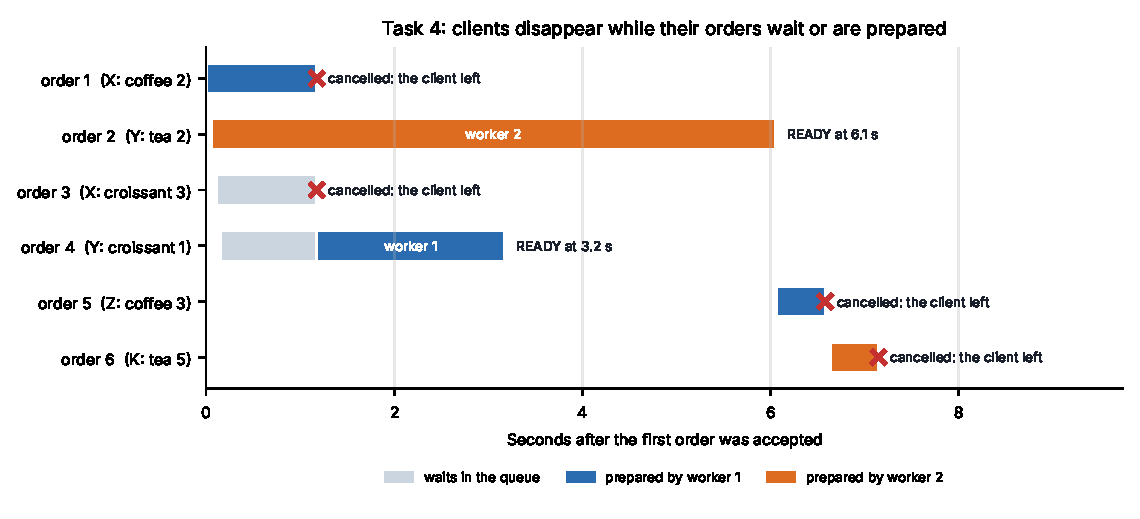
\includegraphics[width=\textwidth]{task4.pdf}
\label{fig:task4}
\end{figure}

\lstinputlisting[style=log,caption={Task 4: the log of the server},label={lst:task4}]{tables/excerpt_task4_server.txt}

The server logged the end of the connection of X \fourCloseMs~ms after the close. Order~1, which a worker was preparing, and order~3, which waited in the queue, were both cancelled, and the menu that Y asked for right after showed their products back in the stock. The worker stopped and took order~4 of Y at once; it was ready \fourFreedSeconds~s after X had left, after its full 2 seconds. Order~2 of Y was not touched. The reset connection was noticed after \fourResetMs~ms and the killed process after \fourKillMs~ms.

\ifnum\netRun=1
The fourth kind of disappearance is the client whose network is gone. The scenario \texttt{network} drops all packets of client X in both directions with a rule of the firewall; nothing is closed and no packet says goodbye. Listing~\ref{lst:network} shows that 3 seconds after the cut the server still believed X to be there (its 10 coffees were still out of the stock) and that the connection ended with the error \textit{timed out} \netSeconds~s after the cut, when the keep-alive questions had stayed without an answer. Then the order was cancelled like in the other cases.

\lstinputlisting[style=log,caption={A client whose network is gone},label={lst:network}]{tables/excerpt_network.txt}
\else
The fourth kind of disappearance, a client whose network is gone, has its own scenario (\texttt{network}), which drops the packets of a client with a rule of the firewall. It needs administrator rights and was not run for this report.
\fi

\subsection{Invalid Input}
\label{sec:invalid}

Listing~\ref{lst:invalid} is the transcript of the scenario \texttt{invalid}. Every wrong message got an error message that says what is wrong: an unknown command, an empty line, a command without parameters, a product without a quantity, a quantity that is not a number or is too large, parameters where none are allowed, and a delivery from a client. A message of 3000 bytes without a line end got one error as soon as it passed 1024 bytes, and after its line end the next message was handled normally. 2000 random bytes were cut at the line ends that happened to be among them and got \badRandomErrors{} error messages. Then the same connection sent 256~KB of random bytes and got \badFloodErrors{} more error messages; meanwhile another client asked for the menu 50 times, and its slowest answer took \badFloodWorstMs~ms. After all of this the server was still running, and the connection that had sent the bytes still worked.

\lstinputlisting[style=log,caption={Invalid input},label={lst:invalid}]{tables/excerpt_invalid.txt}

One more kind of bad client does not send wrong data but never reads the answers (scenario \texttt{never\_reads}, Listing~\ref{lst:mute}). Its receive buffer and the send buffer of the server fill up, and the thread of that connection stops inside \texttt{Send}. Because sending has a limit of 5 seconds, the server gave up after \muteSeconds~s, closed the connection and logged the error; another client was served normally during this time. Without the limit this thread, or a worker that has to send \texttt{READY} to such a client, would be blocked for ever.

\lstinputlisting[style=log,caption={A client that never reads},label={lst:mute}]{tables/excerpt_never_reads.txt}

\subsection{The Console Client}

The scenario \texttt{client\_cs} starts the real console client, lets it order one tea and then leaves its keyboard open without typing anything. \texttt{READY} appeared in its output 3 seconds later, while the program was waiting for the keyboard. Then the server was killed; the client printed the last line of Listing~\ref{lst:client} and ended by itself with exit code 0. The Python client passes the same two checks.

\lstinputlisting[style=log,caption={The output of the console client; the server is killed at the end},label={lst:client}]{tables/excerpt_client_cs.txt}

\subsection{Questions}

\textbf{1. How does your server notice that a client has disappeared? Which kind of disappearance does it notice at once, and which one not?} The thread of the connection is always waiting in \texttt{Receive}, and every kind of disappearance ends this call in its own way (Table~\ref{tab:gone}). A closed connection and a killed process are noticed at once, because the system of the client still tells the server: it sends a FIN or an RST also on behalf of a process that was killed. What is \emph{not} noticed at once is a client that cannot say anything any more: its cable is pulled, its Wi-Fi is gone or its machine lost power. For the server this looks exactly like a client that is thinking. Only the keep-alive of TCP finds it: after 10 seconds of silence the system of the server asks the client whether it is still there, and repeats the question every 5 seconds; after 3 questions without an answer \texttt{Receive} fails. Keep-alive is switched off unless the program asks for it, and with the default times of Linux the first question would come only after two hours.

\begin{table}[H]
  \centering
  \caption{How the server notices a client that disappeared (measured in the scenarios)}
  \renewcommand{\arraystretch}{1.2}
  \small
  \begin{tabular}{>{\raggedright\arraybackslash}p{0.32\textwidth}>{\raggedright\arraybackslash}p{0.38\textwidth}>{\raggedright\arraybackslash}p{0.18\textwidth}}
    \toprule
    \textbf{What happens to the client} & \textbf{What the server sees} & \textbf{Noticed after} \\
    \midrule
    It closes the connection (also \texttt{quit}) & \texttt{Receive} returns 0 & \fourCloseMs~ms \\
    It resets the connection & \texttt{Receive} fails: \textit{connection reset} & \fourResetMs~ms \\
    Its process is killed (\texttt{kill -9}) & \texttt{Receive} returns 0: the system closed the socket & \fourKillMs~ms \\
    Its network is gone & nothing; then \texttt{Receive} fails: \textit{timed out} & \ifnum\netRun=1 \netSeconds~s\else not run\fi \\
    It never reads & \texttt{Send} fails: \textit{timed out}; the server closes & \muteSeconds~s \\
    \bottomrule
  \end{tabular}
  \label{tab:gone}
\end{table}

One limit remains. Keep-alive works on a silent connection. If the server has sent something to the lost client that was never acknowledged (a \texttt{READY}, for example), the system first repeats that data according to its own, longer schedule; we did not measure this case.

\textbf{2. A client disappears while a worker is preparing its order. How does the worker find out and stop, and how do the products get back to the stock?} The worker does not sleep; it waits on the event \texttt{Gone} of the client's connection, for at most the preparation time. When the thread of the connection leaves \texttt{Receive}, it calls \texttt{Shop.Leave}, which, inside the lock, marks every unfinished order of the client as cancelled and adds its products back to the stock; then it sets \texttt{Gone}. The wait of the worker ends at once, the worker asks the shop to finish the order, learns that it is cancelled, writes a line to the log and takes the next order from the queue. The products are returned by the thread of the client, not by the worker; for this reason an order that still waits in the queue returns its products at the same moment, and the worker that meets it later just skips it. The sequence matters: the order is cancelled first and the worker is woken second, so the worker can never wake up and find an order that still looks alive. Nothing of the stopped preparation is kept: the next order that takes these products is prepared for its whole time.

\textbf{3. Why must the client receive and read the keyboard at the same time? How does yours do it?} Both are blocking calls: \texttt{Console.ReadLine} waits for the user and \texttt{Receive} waits for the server, and nobody knows which will have something first. With one thread that waits for the keyboard, a \texttt{READY} or an \texttt{ALERT} would be shown only after the user presses Enter, and the end of the server would not be noticed at all; with one thread that waits for the server, the user could not type. Our client uses two threads: the main thread receives and prints, a second thread reads the keyboard and sends. The second one is a background thread, so when the main thread ends, because the server is gone, the program ends although \texttt{ReadLine} is still waiting. For \texttt{quit} the keyboard thread closes only the sending direction (\texttt{Shutdown}); the server sees the end of the stream and closes its side, the main thread receives 0 and the program ends in the same way. A message that arrives while the user is in the middle of a line is printed in the middle of the typed text on the screen; the typed characters are not lost, and the line is sent when Enter is pressed.

\newpage
\section{Control Questions}
\label{sec:control}

\subsection{Listening Socket and Accepted Sockets}

The listening socket is bound to the port of the server and only receives requests for connections; no message of a client is read from it or written to it. Each \texttt{Accept} returns another socket, connected to exactly one client, and all messages of this client pass through it. With five clients and the provider our server has one listening socket and six accepted sockets, seven in all (and seven threads that wait in them: the main thread in \texttt{Accept} and six in \texttt{Receive}).

\subsection{One Send Is Not One Receive}

TCP carries a stream of bytes and does not remember how the sender grouped them. The bytes of one \texttt{Send} can be cut into several packets, and bytes of several sends can travel together or wait together in the receive buffer until the program reads them; \texttt{Receive} returns what is there at that moment. Our protocol ends every message with \texttt{\textbackslash n}, and the \texttt{MessageReader} of each connection keeps the bytes of an unfinished line between two calls of \texttt{Receive}. Listing~\ref{lst:framing} shows that a message in two pieces, three messages in one send and a message sent byte by byte are all understood correctly.

\subsection{Receive Returns 0, or Fails with a Reset}

\texttt{Receive} returns 0 when the other side has closed its sending direction in the normal way: the stream has ended and no more bytes will come. Data sent before the close has arrived. The error \textit{connection reset} means that the system of the other side has answered with an RST: the connection does not exist there any more, because the program was closed abruptly, the process was killed while data waited unread, or the machine was restarted. Data on the way can be lost. Our server treats both in the same way, as the end of the client, and cancels its orders; only the line in the log differs (Listing~\ref{lst:task4}).

\subsection{The Producer--Consumer Pattern in the Server}

The producers are the threads of the clients: after an order was accepted, the thread of its client puts it into the queue (\texttt{Shop.Enqueue}). The consumers are the workers: each of them takes the oldest order (\texttt{Shop.TakeNext}) and waits there while the queue is empty. The queue between them is the \texttt{BlockingCollection<Order>} of the shop. It is what allows the server to answer at once: the producer only adds the order and returns to its client.

\subsection{The Cost of a Thread That Waits for a Client}

A thread blocked in \texttt{Receive} uses no processor time; the system does not schedule it until bytes arrive. It costs memory, for its stack and for the bookkeeping of the system and the runtime, and it counts towards the limits on threads and open sockets of a process. We measured it by connecting idle clients to the server (Table~\ref{tab:idle} and Figure~\ref{fig:measurements}): from 0 to \idleClientsMax{} idle clients the number of threads grew from \idleThreadsZero{} to \idleThreadsMax{}, one for each client (the few threads of the runtime itself come and go), and the memory of the process from \idleMemZero{} to \idleMemMax~MB, on average about \idleKbPerClient~KB for each waiting client. A menu request was answered in well under a millisecond at every step; the differences between the rows of the last column are noise at this scale.

\begin{table}[H]
  \centering
  \caption{The server with idle clients connected}
  \begin{tabular}{rrrr}
\toprule
Idle clients & Threads & Memory (MB) & Menu answered in (ms, median of 101) \\
\midrule
0 & 14 & 31.0 & 0.041 \\
100 & 114 & 38.9 & 0.037 \\
250 & 264 & 44.4 & 0.009 \\
500 & 514 & 50.6 & 0.043 \\
1000 & 1013 & 63.2 & 0.046 \\
\bottomrule
\end{tabular}

  \label{tab:idle}
\end{table}

So 1000 clients that mostly wait are not a problem for this design on this machine. What would change with many more clients, or with 1000 clients that are all active: every socket is an open file of the process, and the system limits their number; the memory grows with every thread; and when many threads become ready at the same time, the system spends time switching between them. A server for tens of thousands of connections does not give each one a thread; it lets one thread watch many sockets (\texttt{Select}) or uses asynchronous operations, where a waiting connection holds no thread at all.

\subsection{A Race Condition That the Locks Prevent}

The last croissant (Task~2) is one example; here is another, between a worker and a client that leaves. Suppose the state of an order were read and written without the lock. (1)~The preparation time of order~5 ends; the worker reads its state: \textit{preparing}, not cancelled. (2)~At this moment the client disconnects; its thread reads the state: \textit{preparing}, so the order must be cancelled. (3)~The thread of the client puts the products of order~5 back into the stock and writes \textit{cancelled}. (4)~The worker, which decided in step 1, writes \textit{ready} and reports the order as prepared. The order was prepared and its products are also back in the stock: the shop now has products that were already used. In our server the worker's check and change (\texttt{Finish}) and the client's cancellation (\texttt{Leave}) both run inside \texttt{lock (gate)}, so one of them is first as a whole. Either the order becomes ready and is removed from the client's list before \texttt{Leave} looks at the list, or it is cancelled and \texttt{Finish} returns \texttt{false}.

\subsection{What Identifies a TCP Connection}

Four values: the address and the port of one side and the address and the port of the other. Five clients on the same machine have the same address and connect to the same address and port of the server, but the system gives each of them a different port of its own when it connects. In the log of the scenario with five clients they were \twoEndpoints. The five accepted sockets of the server all have the local port of the server; when a packet arrives, the system finds the right socket by all four values.

\section{Bonus}
\label{sec:bonus}

\textbf{The stock is saved.} After every change the server writes the stock to a file (\texttt{data/stock.txt}): first to a temporary file, which is then renamed, so the file is never half written. At the start the server reads this file; if it does not exist, or with the option \texttt{-{}-new-stock}, it puts a random amount from 10 to 50 of each product. The scenario \texttt{restart} checks both (Listing~\ref{lst:restart}): a new stock was \texttt{\restartFirst}; after one order and one delivery the server was killed with \texttt{kill -9} and started again, and the stock was \texttt{\restartAfter}, the same as before the kill. Five more starts with \texttt{-{}-new-stock} gave 15 amounts, all from 10 to 50. One limit: the file holds the stock as the menu shows it, so the products of orders that were still in preparation when the server was killed are not returned after the restart.

\lstinputlisting[style=log,caption={The stock survives a restart of the server},label={lst:restart}]{tables/excerpt_restart.txt}

\textbf{Two programming languages.} \texttt{python/client.py} is the client and the provider written in Python with the module \texttt{socket} only, with the same two threads. It works with the C\# server because the protocol is plain text lines. Moreover, all clients of the scenarios in this report are Python sockets talking to the C\# server.

\textbf{Two computers.} The server binds its listening socket to all addresses of the machine (\texttt{IPAddress.Any}), and the client and the provider take the address of the server with \texttt{-{}-host}. The scenarios of this report run on one machine through the loopback interface, so the report contains no measurement between two computers.

\section{Conclusions}

The server does what the four tasks ask, and each requirement was checked against the running server: \checksPassed{} of \checksTotal{} checks passed. The design rests on three decisions. The first is the protocol: one message is one line, and a small reader that keeps the unfinished bytes of a connection makes the borders of the messages independent of how TCP delivers them. The second is the division of the work between threads: the thread of a connection decides at once (it took \oneAnswerMs~ms to accept an order) and a worker does the slow part, with a queue between them, so an order of 11 seconds does not make its client, or anybody else, wait for an answer. The third is that all shared data is in one class behind one lock, with nothing sent to a socket inside it: in \raceOrders{} simultaneous orders for \raceCroissants{} croissants never more than \raceCroissants{} were accepted, and \consDeliveries{} deliveries mixed with \consOrders{} orders left exactly the stock that the arithmetic gives.

The failures of clients showed which of them are easy. A client that closes, resets or is killed is announced by its own system and was noticed almost at once (Table~\ref{tab:gone}). A client that falls silent is not announced by anybody; the server found it only through keep-alive, after \ifnum\netRun=1 \netSeconds\else about 25\fi~s, and a client that does not read was found only through the limit on sending, after \muteSeconds~s. In every case the orders were cancelled and the products returned by one piece of code, run by one thread.

The number of workers turned out to be a rule of the shop and not a limit of the machine: the workers wait, so \workOrders{} orders were ready in \workSecondsOne~s with one worker and in \workSecondsEight~s with eight, on \envLogical{} logical processors. A thread for each connection was cheap at this scale (about \idleKbPerClient~KB for a waiting client, \idleClientsMax{} clients tried). The limits of the work are stated where they belong: the provider is not authenticated, the products of orders in preparation are lost when the server itself is killed, a message that arrives while the user types appears inside the typed line, and all measurements were made on one machine through the loopback interface.

\section{Source Code}

The C\# source code, the scenario script, the data of this report and the report itself are available in the repository:

\begin{center}
  \url{https://github.com/Moisei-D/PR-Labs}
\end{center}

The program is in the folder \texttt{Lab2} and the report in \texttt{Reports/Lab2 Report}. The \texttt{README.md} of the project describes the options and the protocol; the main commands are:

\begin{terminaloutput}
cd Lab2
dotnet build -c Release
dotnet run -c Release -- server --port 5000
dotnet run -c Release -- client --host 127.0.0.1 --port 5000
dotnet run -c Release -- provider --host 127.0.0.1 --port 5000
python3 python/client.py client --port 5000
python3 tests/scenarios.py
\end{terminaloutput}

\end{document}
